\documentclass[xcolor=dvipsnames, xetex,serif]{beamer}
%\documentclass[handout,xetex,serif]{beamer} %ใช้บรรทัดนี้สำหรับปริ้นเอกสาร
\usepackage{color,amsmath,graphics,graphicx}
\usepackage{epsfig,amsfonts,graphics}
\usepackage{mathrsfs,hyperref}
\usepackage{subcaption,float,framed,algorithm2e,hyperref}
%===============================================
\usepackage{fontspec,xltxtra,xunicode}
\defaultfontfeatures{Scale=1.23}
\XeTeXlinebreaklocale “th_TH” % สำหรับตัดคำ
\setmainfont[Scale=1.23]{THSarabunNew}
% 1.23 เท่าคือจาก 12 pt บน LaTeX ให้เท่ากับ 16pt บน Word
%=====================================================
%\usepackage{pgfpages} %ใช้บรรทัดนี้สำหรับปริ้นเอกสาร
%\pgfpagesuselayout{4 on 1}[a4paper,border shrink=5mm,landscape]
%\pgfpagesuselayout{2 on 1}[a4paper,border shrink=5mm]
 %ใช้บรรทัดนี้สำหรับปริ้นเอกสาร

%%%%%%%%%%%%%%% THEOREM Environments %%%%%%%%%% 					
\newtheorem{conjecture}[theorem]{บทคาดการณ์}								
\newtheorem{remark}[theorem]{หมายเหตุ}										
\numberwithin{equation}{section}							
\renewcommand\tablename{ตารางที่}
\renewcommand\figurename{รูปที่}						
\renewcommand{\bibname}{บรรณานุกรม}						
\renewcommand{\indexname}{ดรรชนี}
\setbeamertemplate{caption}[numbered]	
\setbeamertemplate{theorems}[numbered]				
%%%%%%%%%%%%%%%%%%%%%%%%%%%%%%%%%%%%%%%%%%%%%%%

\mode<presentation>{
	\usetheme{Madrid}
	\usecolortheme[named=black]{structure}}
 \title[วิธีเชิงตัวเลขสำหรับต่อเติมภาพ]{\normalsize{ขั้นตอนวิธีเชิงตัวเลขชนิดใหม่สำหรับการต่อเติมภาพที่ใช้การแปรผันรวมกับการประยุกต์สำหรับซ่อมแซมภาพจิตรกรรมไทยโบราณและการลบบทบรรยายจากอนิเมะ\\A new numerical algorithm for TV-based image inpainting with its applications for restoring ancient Thai painting images and removing subtitles from animes}}
 \author[ภัคพล]{ภัคพล พงษ์ทวี}
 \institute[SU]{
 	ภาควิชาคณิตศาสตร์\\
 	มหาวิทยาลัยศิลปากร \\}
 \date[Project Proposal]{การนำเสนอโครงร่างโครงงานวิจัย\\
 	5 ตุลาคม 2561}
 
 \AtBeginSubsection[]{
 	\begin{frame}<beamer>
 		\frametitle{Outlines}
 		\tableofcontents [currentsection,currentsubsection]
 	\end{frame}}
 	%\setbeamertemplate{item}[square]
 	%============================================================================
 	\begin{document}
 		\begin{frame}
 			\titlepage 
 		\end{frame}
 		%\begin{frame} \tableofcontents \end{frame}
 		\section{Introduction}
		\begin{frame}
			ภาพดิจิตัล และการถ่ายภาพดิจิตัล
		\end{frame} 		
		\begin{frame}
			\frametitle{การประมวลผลภาพ}
			\begin{figure}[H]
				\centering
				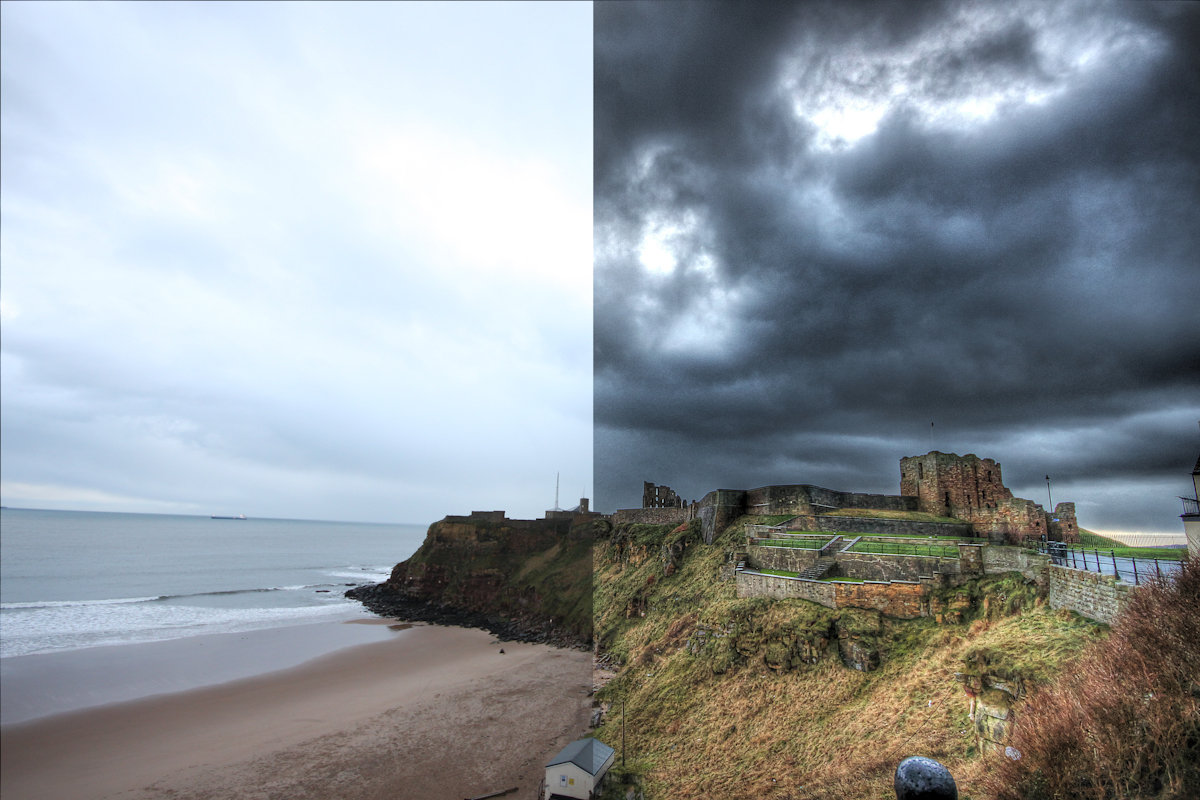
\includegraphics[width=0.6\linewidth]{images/lightroom.jpg}
				\caption{เปรียบเทียบภาพ ก่อน/หลัง การประมวลผล\footnote{ \tiny{ภาพจาก \url{https://commons.wikimedia.org/wiki/File:Before_and_after_HDR_(6747894381).jpg} สืบค้นเมื่อวันที่ 25 กันยายน 2561}}}
				\label{image:lightroom}
			\end{figure}
			%\note{ก่อนภาพจะถูกนำไปใช้ มักจะผ่านการประมวลผลภาพก่อนเสมอ ทั้งภาพตามสื่อสิ่งพิมพ์ต่างๆ ก่อนจะนำไปตีพิมพ์ก็จะนำมาประมวลผลเพื่อให้ได้ภาพที่สวยงาม คมชัดขึ้น หรือแม้กระทั่งภาพทางการแพทย์ก็จะมีการกำจัดสัญญาณรบกวนเพื่อให้สามารถหาสาเหตุของโรคได้ง่ายขึ้่น}
		\end{frame} 		
		\begin{frame}
		\frametitle{การประมวลผลภาพ}
			\begin{figure}[H]
				\centering
				\begin{subfigure}{0.3\linewidth}
					\centering
					
\includegraphics[width=0.8\linewidth]{images/grayscale_inpaint/toinpaint.png}
					\caption{ภาพที่ต้องการซ่อมแซม}
				\end{subfigure}
				\begin{subfigure}{0.3\linewidth}
					\centering
					
\includegraphics[width=0.8\linewidth]{images/grayscale_inpaint/inpaintdomain.png}
					\caption{โดเมนต่อเติม}
				\end{subfigure}
				\begin{subfigure}{0.3\linewidth}
					\centering
					
\includegraphics[width=0.8\linewidth]{images/grayscale_inpaint/result_splitbergman.png}
					\caption{ภาพที่ได้รับการซ่อมแซม}
				\end{subfigure}
				\caption{ตัวอย่างการซ่อมแซมภาพ}
				\label{fig1}
			\end{figure}
		\end{frame} 		
		\begin{frame}
			\frametitle{การประยุกต์ใช้การต่อเติมภาพในปัจจุบัน}
			\begin{figure}[H]
				\centering
				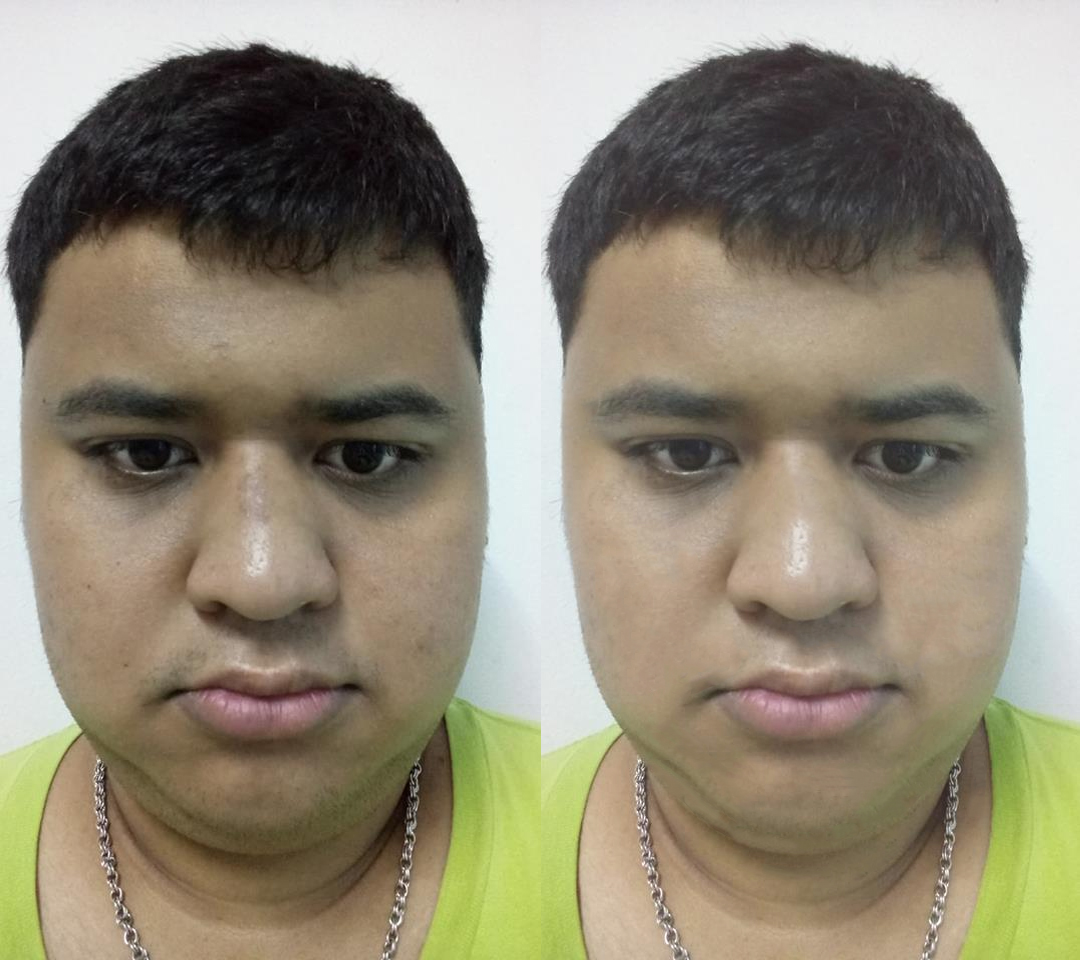
\includegraphics[width=0.6\linewidth]{images/self-beauty.jpg}
				\caption{เปรียบเทียบภาพ ก่อน/หลัง การใช้แอปพลิเคชัน snapseed}
				\label{image:self-beauty}
			\end{figure}
		\end{frame} 		
		\begin{frame}
			\frametitle{การซ่อมแซมภาพจิตรกรรมไทยโบราณ}
			 \begin{figure}[h]
				\[
				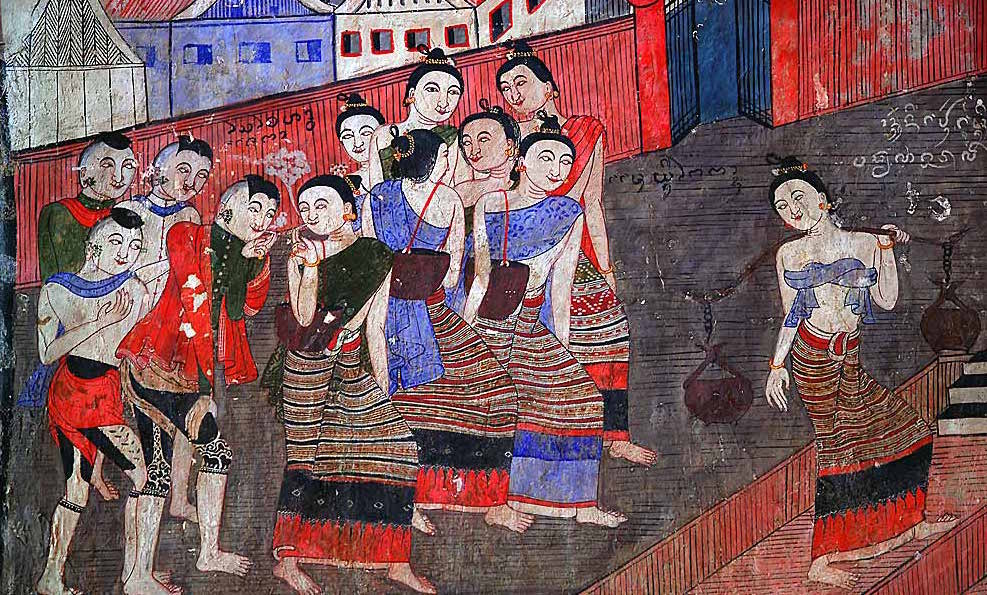
\includegraphics[width=0.6\linewidth]{images/thaiart.jpg}
				\]
				\caption{ภาพจิตรกรรมไทยที่วัดภูมินทร์ อำเภอเมือง จังหวัดน่าน\footnote{\tiny{ภาพถ่ายที่วัดภูมินทร์ อำเภอเมือง จังหวัดน่าน; ภาพจาก \url{http://topicstock.pantip.com/camera/topicstock/2009/02/O7514399/O7514399.html} สืบค้นเมื่อวันที่ 23 กันยายน 2561}}}
				\label{image:thaiart}
			\end{figure}
		\end{frame} 
		\begin{frame}
			\frametitle{การลบบทบรรยายบนอนิเมะ}
			 \begin{figure}[h]
				\[
				
\includegraphics[width=0.6\linewidth]{images/anime-sub.png}
				\]
				\caption{เฟรมของอนิเมะที่มีบทบรรยายแบบแข็ง\footnote{\tiny{ภาพจาก \url{https://www.samehadaku.tv/2018/07/grand-blue-episode-1-subtitle-indonesia.html} สืบค้นเมื่อวันที่ 23 กันยายน 2561}}}
				\label{image:anime-sub}
			\end{figure}
		\end{frame} 
		\begin{frame}
			\frametitle{ความท้าทายในการลบบทบรรยายออกจากอนิเมะ}
			\begin{itemize}
				\item [(1)] อนิเมะเป็นวิดีโอซึ่งแสดงผลประมาณ 24 เฟรม(ภาพ)ต่อวินาที
				\item [(2)] แต่ละเฟรมอาจมีหรืออาจไม่มีบทบรรยายก็ได้
				\item [(3)] แต่ละเฟรมอาจมีหรืออาจไม่มีบทบรรยายเดียวกันก็ได้
				\item [(4)] แต่ละเฟรมเป็นการแสดงผลภาพสีที่มีระดับความคมชัดสูง (high definition) ขนาดมากถึง $1920\times1080$ พิกเซล
			\end{itemize}
		\end{frame} 
		\begin{frame}
			\frametitle{ภาพเฉดเทา}
			\begin{itemize}
				\item โดเมนภาพ (image domain) $\Omega \subset \mathbb{R}^2$ 
				\item โดนเมนต่อเติม
			\end{itemize}
			ให้ $\Omega \subset \mathbb{R}^2$ แทนโดเมนภาพ (image domain) $D \subset \mathbb{R}^2$ แทนโดนเมนต่อเติม (ดูรูปที่ \ref{fig4}) และ $V \subset [0,\infty)$ 
			 \begin{figure}[h]
				\[
				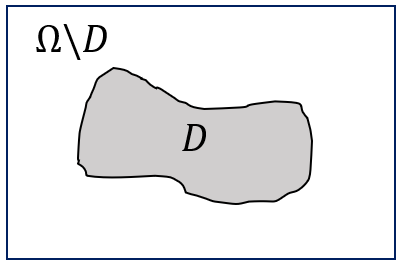
\includegraphics[width=0.3\linewidth]{images/sample-domain.png}
				\]
				\caption{$D$ แทนโดเมนต่อเติม}
				\label{image:sample-domain}
			\end{figure}
		\end{frame} 
		\begin{frame}
			ต่อเติมภาพเฉดเทา
		\end{frame} 
		\begin{frame}
			Explicit Time Marching
		\end{frame} 
		\begin{frame}
			Fix point
		\end{frame} 
		\begin{frame}
			ปัญหา beta
		\end{frame} 
		\begin{frame}
			Split bergman
		\end{frame} 
		\begin{frame}
			Split bergman (3 ขั้น)
		\end{frame} 
		\begin{frame}
			ภาพสี RGB
		\end{frame} 
		\begin{frame}
			แทนเวคเตอร์ในภาพสี
		\end{frame}
		\begin{frame}
			แทนสมการในภาพสี
		\end{frame}
		\begin{frame}
			วัตถุประสงค์
		\end{frame}
		\begin{frame}
			ขอบเขต
		\end{frame}
		\begin{frame}
			วิธีการดำเนินงาน
		\end{frame}
		\begin{frame}
			\centering
			ขอบคุณ
		\end{frame}
		\begin{frame}
		reference (ถ้ามี)
		\end{frame}
	\end{document}





